\section{Dinámica} \label{sec:dinamica}

La dinámica estudia las fuerzas y torques y su efecto en el movimiento del robot. Forma general de la ecuación dinámica es: 
 
\begin{figure}[h]
	\centering
	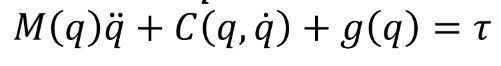
\includegraphics[width=0.5\linewidth]{img/ECDINA}
	\caption{Ecuación dinámica}
	\label{fig:ECDINA}
\end{figure} 
 
  donde:
  q: Coordenadas articulares generalizadas\\[5pt]
  M(q): Matriz de masa o inercia\\[5pt]
  C(q,q’):Fuerzas centrífugas y de Coriolis\\[5pt]
  g(q): Fuerzas de gravedad\\[5pt]
  torque = Fuerzas (o pares) generalizadas\\[5pt]
  

\subsection{Matriz de masa o inercia}


La matriz de masa M(q) representa cómo la masa del robot está distribuida y cómo esa masa influye en la resistencia al movimiento. Es una matriz simétrica y positiva definida la cual depende de la configuración q del robot y está formada por los parámetros físicos del sistema, como: \\[5pt]
-Las masas de los eslabones \\[5pt]
-Longitudes de los brazos \\[5pt]
-Momentos de inercia de cada segmento. \\[5pt]

Esta matriz se obtiene a partir del modelo dinámico del robot usando el método de Euler-Lagrange y no solo describe la resistencia al movimiento sino también define el límite superior de la aceleración que puede alcanzar un robot bajo una cantidad de fuerza o torque. Esto nos indica que a mayor inercia menor será la aceleración máxima que puede lograrse con un mismo torque. 

\subsection{Matriz de coriolis}

La matriz de Coriolis representa los efectos que causan las fuerzas centrífugas y fuerzas de Coriolis las cuales surgen cuando el robot se encuentra en movimiento. Estas fuerzas aparecen debido a las velocidades articulares y depende de la posición y velocidad. 
Se basa en derivadas parciales de la matriz de inercia y se utilizan los coeficientes de Christoffel. 

\subsection{Vector de gravedad}

El vector de gravedad representa las fuerzas que ejercen el peso en los eslabones dependiendo de su configuración. Cuando el robot está extendido horizontalmente, el torque necesario para mantener su propio peso es el máximo ya que se necesita más torque para sostener el peso de los eslabones que están más alejados del eje del motor. 

\subsection{Fricción}

La fricción es la fuerza que se opone al movimiento entre dos superficies que se encuentran en contacto.

\subsubsection{Fricción estática o seca}

Es la fuerza la cual impide el movimiento de un objeto en contacto con otro objeto o superficie. La velocidad debe ser igual a 0.
 
\subsubsection{Fricción dinámica o viscosa}

Es la fuerza que se opone al movimiento cuando el objeto  ya está en  movimiento. La velocidad es diferente a cero. 



\subsection{Perturbaciones}
Una perturbación es cualquier fenómeno que causa un cambio o alteración en el comportamiento de un sistema. 
